% Fields between Q and Q(zeta_20): the Hilbert class field of Q(sqrt(-5)) (drawn by hand).
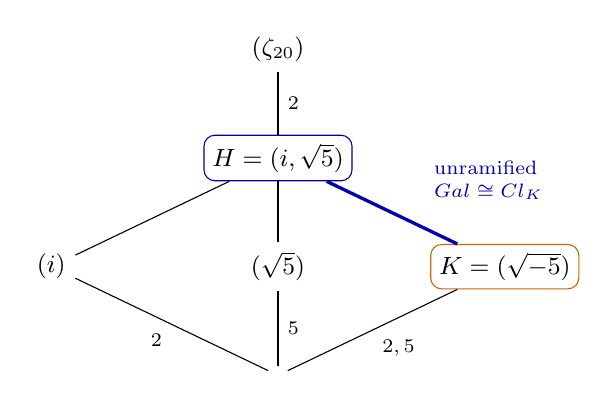
\begin{tikzpicture}[x=1.2cm,y=1.15cm,every node/.style={font=\small}]
\node (Z) at (0,3.6) {$\Q(\zeta_{20})$};
\node[draw=blue!70!black,rounded corners,inner sep=3pt] (H) at (0,2.4) {$H=\Q(i,\sqrt5)$};
\node (i) at (-2.4,1.2) {$\Q(i)$};
\node (s5) at (0,1.2) {$\Q(\sqrt5)$};
\node[draw=orange!80!black,rounded corners,inner sep=3pt] (K) at (2.4,1.2) {$K=\Q(\sqrt{-5})$};
\node (Q) at (0,0) {$\Q$};
\draw (Z)--node[right,font=\scriptsize]{$2$}(H);
\draw (H)--(i); \draw (H)--(s5);
\draw[blue!70!black,very thick] (H)--(K);
\node[blue!70!black,font=\scriptsize,align=left,anchor=west] at (1.55,2.15) {unramified\\$\operatorname{Gal}\cong\operatorname{Cl}_K$};
\draw (Q)--node[below left,font=\scriptsize]{$2$}(i);
\draw (Q)--node[right,font=\scriptsize]{$5$}(s5);
\draw (Q)--node[below right,font=\scriptsize]{$2,5$}(K);
\end{tikzpicture}
